\begin{figure}[H]
	\begin{center}
		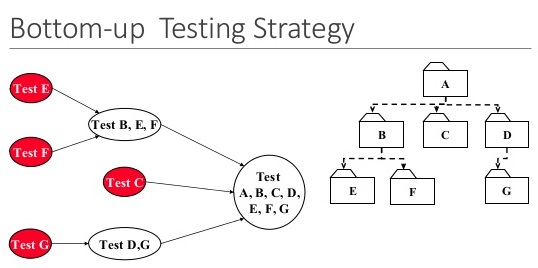
\includegraphics[width=\textwidth]{./DD_Diagrams/testplan2.jpg}
      \caption{Bottom up- strategy for testing integration plan}
        \label{TrackMe_tp2}
	\end{center}
\end{figure}
A bottom-up approach is the piecing together of systems to give rise to more complex systems, thus making the original systems sub-systems of the emergent system. Bottom-up processing is a type of information processing based on incoming data from the environment to form a perception. From a cognitive psychology perspective, information enters the eyes in one direction (sensory input, or the "bottom"), and is then turned into an image by the brain that can be interpreted and recognized as a perception (output that is "built up" from processing to final cognition). In a bottom-up approach the individual base elements of the system are first specified in great detail. These elements are then linked together to form larger subsystems, which then in turn are linked, sometimes in many levels, until a complete top-level system is formed. This strategy often resembles a "seed" model, by which the beginnings are small but eventually grow in complexity and completeness. However, "organic strategies" may result in a tangle of elements and subsystems, developed in isolation and subject to local optimization as opposed to meeting a global purpose.\newline
Considering the implementation plan and the overall architecture of the TrackMe application, the chosen strategy for the integration testing is the \textit{bottom-up strategy}. This allows us to start the integration and it’s testing while not waiting for the completion of the development and the unit testing of each component in the system. Considering the integration of two components, we would assume that, in best case, they have been implemented fully and that their respectful unit tests pass. However, the integration can, in some cases, start, if necessary, before the implementation has been completed. This can be allowed if the part of the component needed for that specific integration has been completed and tested. \newline

Since the opted solution is to start from the bottom-up, that means that the among the first integrations performed will have the already built external components in them. Since the application rests on these services and the communication with them, this order of integration and testing will enable the earlier detection of errors in these critical parts. 
\begin{figure}[H]
	\begin{center}
		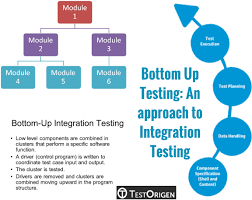
\includegraphics[width=\textwidth]{./DD_Diagrams/testplan.png}
      \caption{Working of bottom up- strategy for testing integration plan}
        \label{TrackMe_tp}
	\end{center}
\end{figure}